%%%%%%%%%%%%%%%%%%%%%%%%%%%%%%%%%%%%%%%%%%%%%%%%%%%%%%%%%%%%%%%%%%%%%%%%%%%%%%%%
%2345678901234567890123456789012345678901234567890123456789012345678901234567890
%        1         2         3         4         5         6         7         8

\documentclass[letterpaper, 10 pt, conference]{ieeeconf}  % Comment this line out
                                                          % if you need a4paper
%\documentclass[a4paper, 10pt, conference]{ieeeconf}      % Use this line for a4
                                                          % paper

\IEEEoverridecommandlockouts                              % This command is only
                                                          % needed if you want to
                                                          % use the \thanks command
\overrideIEEEmargins
% See the \addtolength command later in the file to balance the column lengths
% on the last page of the document
\usepackage[utf8]{inputenc}
\usepackage[usenames]{color}
\usepackage{amssymb, amsmath, amsbsy}
\usepackage{amsfonts}
\usepackage{mathrsfs,amsmath} 
\usepackage{multirow}
\usepackage{lscape}
\usepackage[spanish]{babel}
\selectlanguage{spanish}
\providecommand{\abs}[1]{\lvert#1\rvert}
\providecommand{\norm}[1]{\lVert#1\rVert}

\usepackage[utf8]{inputenc}
\usepackage[T1]{fontenc}

% The following packages can be found on http:\\www.ctan.org
\usepackage{graphics} % for pdf, bitmapped graphics files
\usepackage{epsfig} % for postscript graphics files
\usepackage{mathptmx} % assumes new font selection scheme installed
\usepackage{times} % assumes new font selection scheme installed
\usepackage{amsmath} % assumes amsmath package installed
\usepackage{amssymb}  % assumes amsmath package installed
\usepackage{color}
\definecolor{gray97}{gray}{.97}
\definecolor{gray75}{gray}{.75}
\definecolor{gray45}{gray}{.45}
\usepackage{listings} 
% \begin{lstlistings} [language=<language>]
% accepted languages: ABAP, ACSL, Ada, Algol, Ant, Assembler, Awk, bash, Basic, C#, C++, C, Caml, Clean, Cobol, Comal, csh, Delphi, Eiffel, Elan, erlang, Euphoria, Fortran, GCL, Gnuplot, Haskell, HTML, IDL4, inform, Java, JVMIS, ksh, Lisp4, Logo, Lua, make, Mathematica, Matlab, Mercury, MetaPost, Miranda, Mizar, ML, Modelica, Modula-, MuPAD, NASTRAN, Oberon-, Objective C , OCL, Octave, Oz, Pascal, Perl, PHP, PL/I, Plasm, POV, Prolog, Promela, Python, R, Reduce, Rexx, RSL, Ruby, S4, SAS, Scilab, sh, SHELXL, Simula, SQL, tcl, TeX, VBScript, Verilog, VHDL, VRML, XML, XSLT.

\usepackage{minted}
 \renewcommand\listoflistingscaption{Lista de fragmentos de códigos}
\renewcommand\listingscaption{Código}

%\usepackage{listings}
%\lstset{ frame=Ltb,
%framerule=0pt,
%aboveskip=0.5cm,
%framextopmargin=3pt,
%framexbottommargin=3pt,
%framexleftmargin=0.4cm,
%framesep=0pt,
%rulesep=.4pt,
%backgroundcolor=\color{gray97},
%rulesepcolor=\color{black},
%
%stringstyle=\ttfamily,
%showstringspaces = false,
%basicstyle=\small\ttfamily,
%commentstyle=\color{gray45},
%keywordstyle=\bfseries,
%%
%numbers=left,
%numbersep=15pt,
%numberstyle=\tiny,
%numberfirstline = false,
%breaklines=true,
%}

% minimizar fragmentado de listados
\lstnewenvironment{listing}[1][]
{\lstset{#1}\pagebreak[0]}{\pagebreak[0]}

\lstdefinestyle{consola}
{basicstyle=\scriptsize\bf\ttfamily,
backgroundcolor=\color{gray75},
}
\lstdefinestyle{R}
{language=R,
}










%\usepackage[svgnames]{xcolor}
%\usepackage{listings}
% \begin{lstlistings} [language=<language>]
% accepted languages: ABAP, ACSL, Ada, Algol, Ant, Assembler, Awk, bash, Basic, C#, C++, C, Caml, Clean, Cobol, Comal, csh, Delphi, Eiffel, Elan, erlang, Euphoria, Fortran, GCL, Gnuplot, Haskell, HTML, IDL4, inform, Java, JVMIS, ksh, Lisp4, Logo, Lua, make, Mathematica, Matlab, Mercury, MetaPost, Miranda, Mizar, ML, Modelica, Modula-, MuPAD, NASTRAN, Oberon-, Objective C , OCL, Octave, Oz, Pascal, Perl, PHP, PL/I, Plasm, POV, Prolog, Promela, Python, R, Reduce, Rexx, RSL, Ruby, S4, SAS, Scilab, sh, SHELXL, Simula, SQL, tcl, TeX, VBScript, Verilog, VHDL, VRML, XML, XSLT.

%\usepackage{minted}
% \renewcommand\listoflistingscaption{Lista de fragmentos de códigos}
%\renewcommand\listingscaption{Código}
%\title{}

\makeatletter
\let\thetitle\@title
\makeatother


\title{\LARGE \bf
Martingalas: el teorema de parada de martingalas, la desigualdad de Wald y la desigualdad de Azuma-Hoeffding*'**
}

%\author{ \parbox{3 in}{\centering Huibert Kwakernaak*
%         \thanks{*Use the $\backslash$thanks command to put information here}\\
%         Faculty of Electrical Engineering, Mathematics and Computer Science\\
%         University of Twente\\
%         7500 AE Enschede, The Netherlands\\
%         {\tt\small h.kwakernaak@autsubmit.com}}
%         \hspace*{ 0.5 in}
%         \parbox{3 in}{ \centering Pradeep Misra**
%         \thanks{**The footnote marks may be inserted manually}\\
%        Department of Electrical Engineering \\
%         Wright State University\\
%         Dayton, OH 45435, USA\\
%         {\tt\small pmisra@cs.wright.edu}}
%}

\author{Morante Moran David Willians$^{1}$, Valdivia Fuentes Juan Daniel$^{2}$, Geronimo Aparicio Mirian Andrea$^{3}$\\
 \small Universidad Nacional de Ingeniería - Facultad de Ciencias - Escuela profesional de Matemática
\thanks{*Procesos Estocásticos}% <-this % stops a space
\thanks{*Trabajo colaborativo disponible en Github}
\thanks{$^{1}$Morante Moran David - 20170333E - Escuela profesional de Matemática
        }%
\thanks{$^{2}$Valdivia Fuentes Juan Daniel -20162677K - Escuela profesional de Matemática
        }%
 \thanks{$^{3}$Geronimo Aparicio Mirian - 20172192J - Escuela profesional de Matemática
      }%
}


\begin{document}



\maketitle
\thispagestyle{empty}
\pagestyle{empty}


%%%%%%%%%%%%%%%%%%%%%%%%%%%%%%%%%%%%%%%%%%%%%%%%%%%%%%%%%%%%%%%%%%%%%%%%%%%%%%%%
\begin{abstract}
 Se hablará de los procesos estocásticos, que sirven para usar magnitudes aleatorias que varían con el tiempo o para caracterizar una sucesión de variables aleatorias (estocásticas) que evolucionan en función de otra variable, generalmente el tiempo.
Tambien  estudiamos los teoremas y desigualdades en la cual intervienen las martingalas, una vez entendido eso trataremos problemas y aplicaciones interesantes que se presentan con mayor frecuencia en la vida cotidiana, dándoles una solución y  integrandole a ello el uso del lenguaje R.

\end{abstract}


%%%%%%%%%%%%%%%%%%%%%%%%%%%%%%%%%%%%%%%%%%%%%%%%%%%%%%%%%%%%%%%%%%%%%%%%%%%%%%%
\begin{center}
   \bf{INTRODUCCIÓN}
\end{center}
\label{sec:1}
Dando un preámbulo a lo que será una definición formal, las martingalas son procesos estocásticos que modelan juegos justos; en promedio no se pierde ni se gana en la siguiente observación del proceso.\\

Existen muchos problemas interesantes a tratar relacionados a este proceso estocástico, en este artículo abordaremos  en particular  el problema conocido como "La ruina del jugador", en el cual se utilizará el teorema de parada para martingalas acotadas y las martingalas.\\

El objetivo de este estudio es  explicar y enfatizar más la teoría de probabilidades  y desarrollar algun algoritmo y códigos en R que faciliten la comprensión teórica desde el punto de vista de la ciencia computacional. \\

Para ello  en la sección \ref{sec:2.1} partiremos definiendo los conceptos de \textit{Filtración} y \textit{Esperanza condiocional} para asi definir  en la sección \ref{sec:2.2} lo que es una \textit{Martingala} junto con sus teoremas y propiedades elementales. Luego de tener una vision amplia se abordará en la sección \ref{sec:2.3} los\textit{ Tiempos de paradas} para luego enunciar el \textit{Teorema de paradas para martingalas acotadas}, dando como ejemplo lo que es un camino aleatorio simple. Conceptos que son necesarios para abordar los dos teoremas y el problema aplicativo  sobre el que versará el trabajo. En el Desarrollo del experimento mostraremos las técnicas, y las propiedades que utilizamos para obtener asi la demostracion de los teoremas, finalizando con la implementación del código R y la reproducción de resultados reportados en dos artículo científico relacionados con Cadenas de Markov y la estrategia de la Martingala.
\newpage
\begin{center}\label{sec:2}
    \bf{ DEFINICIONES}
\end{center}
\section{Filtración}
Una filtración \(\mathbb{F}\) es un conjunto indexado \(\mathcal{F}_{i}\) de subestructuras de una estructura algebraica \(\mathcal{F}\), recorriendo el subíndice i cierto conjunto I conjunto totalmente ordenado cumpliendo la condición:
\begin{center}
    $
\forall i,j \in I : i\leq j \Rightarrow \mathcal{F}_{i} \subseteq \mathcal{F}_{j} $
\end{center}


si el indice i es el parámetro tiempo de un proceso estocástico entonces la filtración puede interpretarse como una representación de todo el histórico de información hasta el instante dado.
\section{Esperanza condicional}\label{sec:2.1}
Sea ($\Omega$,$\mathcal{F}$,$\mathbb{P}$) un espacio de probabilidad, con una variable aleatoria  X:$\Omega$ \xrightarrow{} \(\mathbb{R}^{n}\) y un sub-$\sigma$-algebra \\
A continuación, una esperanza condicional de X dado por $\mathcal{H}$ (denotado como  $\mathbb{E}$ [X|$\mathcal{F}$]) es cualquier $\mathcal{H}$- función medible ($\Omega$ \xrightarrow{} $\mathbb{R}^{n}$) que satisface : \\

\begin{equation*}
\int_{H}^{} \mathbb{E} [X|\mathcal{F}] d\mathbb{P}(\omega) = \int_{H}^{} X(\omega) d \mathbb{P}(\omega)
\end{equation*}

para cada H $\in$ \(\mathcal{H}\). \\
Tenga en cuenta que $\mathbb{E}$ [X|$\mathcal{H}$] es simplemente el nombre de la función esperanza condicional.


\section{Martingala}\label{sec:2.2}
Una definición básica de una martingala de tiempo discreto es un proceso estocástico de tiempo discreto (es decir, una secuencia de variables aleatorias)$ X_{1}, X_{2}, X_{3}$, ... que satisface para cualquier momento n:
\begin{itemize}
\item \(\mathbb{E}\)($|X_{n}$|)< $\infty$
\item \(\mathbb{E}\)($X_{n+1}|X_{1},...,X_{n}$)=$X_{n}$
\end{itemize}
Es decir, el valor esperado condicional de la siguiente observación, dadas todas las observaciones anteriores, es igual a la observación más reciente.\\
\section{ Martingala con respecto a otra secuencia}
De manera más general, se dice que una secuencia$ Y_{1}, Y_{2}, Y_{3} $... es una martingala con respecto a otra secuencia  $X_{1}, X_{2}, X_{3}$, ... si para todo n.
\begin{itemize}
\item \(\mathbb{E}\)($|X_{n}$|) < $\infty$
\item \(\mathbb{E}\)($Y_{n+1}|X_{1},...,X_{n}$)=$Y_{n}$
\end{itemize}
Del mismo modo, una martingala de tiempo continuo con respecto al proceso estocástico X(t) es un proceso estocástico Y(t) tal que para todo t
\begin{itemize}
\item \(\mathbb{E}\)($|Y_{n}$|) < $\infty$
\item \(\mathbb{E}\)($Y_{t}|{X_{\tau},\tau \leq s} $)=$Y_{s}$ , $\forall s \leq t$.
\end{itemize}
Esto expresa la propiedad de que la expectativa condicional de una observación en el tiempo t, dadas todas las observaciones hasta el tiempo \textit{s}, es igual a la observación en el tiempo s (por supuesto, siempre que \textit{s} $\leq$ \textit{t}). Ademas $Y_{n}$ es medible con respecto a $X_{1},...,X_{n}$.

\section{Definición general}
Sea un espacio de probabilidad ($\Omega$,\(\mathcal{F}\),\(\mathbb{P}\)).
Sea \(\mathbb{F}\) una filtración de $\sigma$-algebras:
$
\mathcal{F}_{1}  \subset ...  \subset \mathcal{F}_{t}\subseteq \mathcal{F}$

Sea ${X(t)}=X_{1},X_{2},...,X_{n}$ una sucesion de variables aleatorias que forman un proceso estocástico.\\
Entonces el proceso estocástico ${X(t),t\geq0}$ adaptado a la filtración \(\mathbb{F}\) recibe el nombre de martingala si :

\begin{equation*}
\mathbb{E} [X(t)|\mathcal{F}_{s}] = X(s)
\end{equation*} Esto es, un proceso estocástico es una martingala cuando su esperanza en tiempo futuro es precisamente el valor que la variable tiene en tiempo presente. Esto significa que el proceso no tiene deriva estadística.



\section{Tiempos de paradas}\label{sec:2.3}
Sea {$Y_{n}$} una supermartingala con respecto a $X_{n}$, y sea $H_{n}$ una función de $(X_{0},X_{1},...,X_{n})$ que cumple 0 $ \leq H_{n} \leq  c_{n}$.Entonces:
\begin{equation*}
W_{n}= W_{0} + \sum_{m=1}^{n} H_{m}(Y_{m}-Y_{m-1})
\end{equation*} , es una supermartingala. La interpretación de esto es que si un juego es desfavorable seguirá siendolo independientemente de cómo apostemos en cada momento. Decimos que \textbf{T} es un \textbf{tiempo de parada} respecto a $X_{n}$ cuando la ourrencia o no del suceso "paramos en el instante n"  \textbf{(T=n)} se puede determinar apartir de los valores 
$X_{0},X_{1},...,X_{n}$.
\subsubsection{Propiedades} Tiempos de paradas\\
Denotemos \textbf{$T \wedge n$} el mı́nimo de T y n.
Si $Y_{n}$ es una martingala con respecto a $X_{n} $ y \textbf{T} es un tiempo de parada con respecto a $X_{n} $ , entonces el proceso (truncado) $Y_{T\wedge n} $ es una martingala con respecto a $X_{n}$


\section{  Teorema de paradas para martingalas acotadas}
Sea $M_{n}$ una martingala con respecto a $X_{n} $ , y sea \textbf{T} un
tiempo de parada con respecto a $X_{n} $, con \(\mathbb{P}\)(\textbf{T} < $\infty$) = 1. Si
existe una constante \textit{k} de manera que $|M_{T\wedge n}| \leq \textit{k}$,  $\forall$ \textit{s},entonces:
\begin{equation*}
\mathbb{E} (M_{T}) = \mathbb{E} (M_{0})
\end{equation*}
La idea bajo la condición $|M_{T\wedge n}| \leq \textit{k}$ para algún \textit{k} es que la
cantidad de dinero disponible es limitada. En caso contrario,
podrían darse situaciones en las que aplicando un criterio de
parada tengamos siempre una ganancia.\\
\newpage
\begin{center}
\bf{PROBLEMAS GENERALES}
\end{center}
 \section*{ I. Desigualdad de Azuma-Hoeffding}
Supongamos que $X_{n},  n\geq 1$ es una martingala tal que $X_{0}=0$ y $\abs{X_{i}-X_{i-1}}\leq d_{i}, 1\leq i\leq n $ para algunas constantes $d_{i}, 1\leq i \leq n$. Luego para todo $t>0,$\\
\begin{equation*}
  \mathbb{P}(\abs{X_{n}}>t)\leq 2 exp\left(\frac{-t^{2}}{2\sum_{i=1}^{n}{d_{i}}^{2}}\right)
  
\end{equation*}
    Tenga en cuenta que en el caso especial cuando $d_{i} = d$, podemos tomar $t = xn$ y obtener
$p$ un límite superior $2 exp(\frac{-x^{2n}}{2d^{2}})$ - que tiene la forma prometida anteriormente.
Tenga en cuenta que esto es coherente con el Chernoff vinculado para el caso especial $X_{n}$ es
la suma de i.i.d. términos de media cero, aunque es aplicable solo en el caso especial
de incrementos acotados.
\section*{II. Lema de Wald}\label{sec:2.5}
  %  Consideremos ahora un camino aleatorio $S_{n}=S_{0}+\xi_{1}+...+\xi_{n}$, donde $\left\lbrace{{\xi_{n}}}\right\rbrace_{n}$ son variables i.i.d. Supongamos que $\mu=E(\xi_{i})<\infty.$ Entonces $M_{n}=S_{n}-n\mu$ es una martingala respecto a $S_{n}$ .
   %  \begin{itemize}
    %     \item Si $T$ es un tiempo de parada con $E(T)<\infty$, entonces $E(S_{T}-L_{0})=\mu E(T)$.
     %\end{itemize}
     %Teniendo esto en cuenta, si consideramos un juego con ganacia $1$ con probabilidad $p$ y $y-1$ con probabilidad $1-p>p$, y comenzamos con $x$ euros, el tiempo medio en perderlo todo $(E_{x}V_{0})$ seria $\frac{x}{1-p}$.
     
     Una variabale aleatoria N que toma valores en los enteros no negativos es un "tiempo de paro " con respecto a ${X_{n}}$ si la ocurrencia (o no ocurrencia) del evento $[N=n]$ puede determinarse observando las variables $X_{1}, X_{2}, X_{3},..., X_{n}$. Por ejemeplo suponga ${X_{n}}$ son v.a aleatorias independientes tales que $$P=[X_{n}=0]=P[X_{n}=1]=\frac{1}{2}  ,  n=1,2,3,...,n$$ Entonces, la variable $$N=min\lbrace{n:X_{1}+ X_{2}+ X_{3}+...+ X_{n}=10}\rbrace$$ es un tiempo de paro con respecto $X_{n}$\\
     (Lema de wald). Si $X_{1}, X_{2}, X_{3}...$ son variables independientes e identicamente distribuidas con esperanza finita y $N$ es un tiempo de paro con respecto a esta sucesion de variables tal que $EN< \infty$, entonces $$E\sum_t^{N}X_{i}=EN.EX$$ 
         

\section*{ III. "La ruina del jugador"}\label{sec:2.4}
 Dicho problema consiste en calcular la probabilidad de que un jugador arruine al contrario en un juego a un número indeterminado de partidas, cuando los dos jugadores inician el juego con un cierto número de monedas cada uno.\\ \\
 
 Sea $S_{n}=S_{0}+\xi_{1}+...+\xi_{n}$, donde $\xi_{i}$ son i.i.d con \(\mathbb{P}\)$(\xi_{i}=1)=p$ y \(\mathbb{P}\)$(\xi_{i}=-1)=q:=1-p$. Ya hemos visto que g$($S_{n}$)_{n}$ es una martingala para g(x)=$(\frac{q}{p})^{x}$. \\ Sea T= min$\left\lbrace n : S_{n} \not\in (a,b) \right\rbrace$ \\
 \begin{itemize}
\item T es un tiempo de parada
\item \(\mathbb{P}\)($ T < \infty$)=1.
\item Si $S_{0}=x$, se cumple $(q/p)^{x}=(q/p)^{a}+[(q/p)^{b}-(q/p)^{a}]\mathbb{P}(S_{T}=b)$
\end{itemize}\
Si definimos $V_{y}$ = min$\left\lbrace   n \leq 0 : S_{n} = y  \right\rbrace$.\\
\begin{equation*}
    \mathbb{P}_{x}(V_{b}<V_{a})=\dfrac{(q/p)^{x}-(q/p)^{a}}{(q/p)^{b}-(q/p)^{a}}
\end{equation*}


 
 


     

     
\begin{center}
    \bf{ESTADO DEL ARTE}
\end{center}
Algunos artículos que hablan sobre el problema de la ruina del jugador, la ruleta  y el estudio de las martingalas y la utilización de sus propiedades.
\begin{itemize}
    \item Cadenas de Markov: Estudio sobre el problema de la ruina del jugador, Autor: Marc Martínez, Universitat autònoma de Barcelona, Encontró mediante diferentes
maneras de plantear la estrategia de
la Martingala, el juego que mejor se adapte
a las necesidades del jugador, en este
caso  dos opciones o bien ampliar
la duración del juego o aumentar la probabilidad
de ganancia. Mediante cálculo de probabilidades
y los procesos de simulación con
código R,sirvieron para encontrar
la situación más favorable en el problema.
 \item PORTILLA, LILIANA MARGARITA; ARIAS MONTOYA, LEONEL; FERNÁNDEZ HENAO, SERGIO
AUGUSTO
,MARTINGALAS Y EL JUEGO DE LA RULETA,
Scientia Et Technica, vol. XV, núm. 43, diciembre, 2009, pp. 124-129
,Universidad Tecnológica de Pereira,En este trabajo se habló sobre el juego de la ruleta bajo el concepto de los
procesos estocásticos, más específicamente sobre la martingala, ya que va muy
relacionada con esta temática estocástica. Seguidamente se muestra un ejemplo
de apuestas donde un jugador intenta ganarle a otro que nunca se rinde, lanzando
una moneda al aire y apostando por la cara, de está manera mediante una
simulación se observa el comportamiento de este tipo de apuestas, bajo el
concepto de las martingalas, también se analiza los efectos presentados al
cambiar los montos iniciales de apuesta y el trabajar con una moneda balanceada
y otra desbalanceada. Este ejemplo es simulado con un código creado en el
software R, el cual muestra el comportamiento de la apuesta y se puede observar
como varía la posibilidad de ganar o perder, que en este caso tiene un tiempo t
para cuando el jugador gana 10 pesos o se queda sin dinero para apostar.
Pereira, Colombia
\end{itemize}

\begin{center}
   \textbf{DISEÑO DEL EXPERIMENTO}
\end{center}
%ESCRIBIR LAS TECNICAS UTILIZADAS ÝA SEA PARA EL CODIGO O PARA LAS DEMOSTRACIONES


%Se busca probar la desigualdad de Wald, la desigualdad de Azuma-Hoeffding y a su vez implementar un código en lenguaje R sobre el famoso problema de la ruina del jugador, para tener bien claro el procedimiento a seguir se deben utilizar las siguientes tecnicas
\begin{itemize}
    \item Para demostrar la desigualdad de Azuma se utilizará la convexidad de la función exponencial ,y su representación como serie infinita de potencias asi como tambien se utilizará algunas estimaciones de la funcion factorial y la función exponencial.
    \item Una de las propiedades de la esperanza condicional que se utiliza para la demostración de la desigualdad de Azuma :\\ Si X es una v.a integrable con $\mathcal{G}\subset \mathcal{F}$ entonces \[\mathbb{E}[\mathbb{E}(X|\mathcal{G})]=\mathbb{E}(X)\]
    \item Teorema de la convergencia monotona
    \item teorema de parada de martingalas en la demostracion del lema de Wald

    
\end{itemize}

\begin{center}
\textbf{EXPERIMENTO Y RESULTADO}
\end{center}
\section*{I. PRUEBA(desigualda de Azuma-Hoeffding)}
$f(x)= exp(\lambda x)$ es una función convexa en $x$ para cualquier$\lambda \in \mathbb{R}$.
Entonces tenemos $f(-d_{i}) = exp (-\lambda d_{i})$ y $f(-d_{i}) = exp (\lambda d_{i})$ .
Usando convexidad tenemos que cuando $\abs{x/d_{i}}\leq 1$
\[ exp(\lambda x) = f(x)=f\left(\dfrac{1}{2}( \dfrac{x}{d_{i}}+1)(d_{i})+\dfrac{1}{2}( 1-\dfrac{x}{d_{i}})(-d_{i})\right) 
\]
utilizando una propiedad de convexidad de la función exponencial tenemos luego que :
\[ f(x)\leq  \dfrac{1}{2}\left(\dfrac{x}{d_{i}}+1\right)f(d_{i})+\dfrac{1}{2}\left(1-\dfrac{x}{d_{i}}\right)f(-d_{i})
\]
\begin{equation}
    = \dfrac{f(d_{i})+f(-d_{i})}{2}+\dfrac{f(d_{i})-f(-d_{i})}{2}x
\end{equation}
Además, para cada $a$
\[ \dfrac{exp(a)+exp(-a)}{2}= \displaystyle\sum_{k=0}^{\infty}\dfrac{a^{k}}{k!}+\displaystyle\sum_{k=0}^{\infty}\dfrac{(-1)^{k}a^{k}}{k!}=\displaystyle\sum_{k=0}^{\infty}\dfrac{a^{2k}}{(2k)!}
\]
\begin{center}
  $ \hspace{2.3cm}\leq \displaystyle\sum_{k=0}^{\infty}\dfrac{a^{2k}}{2^{k}k!}$  (porque $2^{k}k!\leq(2k)!$)
\end{center} 
\begin{equation}
   \hspace{0.99cm} = \displaystyle\sum_{k=0}^{\infty}\dfrac{(\frac{a^2}{2})^{k}}{k!}= exp(\frac{a^2}{2}). 
\end{equation}

Concluimos que por cada x tal que $\abs{x/d_{i}}\leq 1$
\begin{equation}
    exp(\lambda x) \leq exp(\dfrac{d_{i}^{2}}{2}) + \dfrac{exp(\lambda d_{i})-exp(-\lambda d_{i})}{2}
\end{equation}

Ahora pasamos a nuestra secuencia de martingala $X_{n}$.Para cada $t>0$ y cada $\lambda> 0$ tenemos
\[ 
\mathbb{P}(X_{n})=\mathbb{P}(exp(\lambda X_{n})\geq exp(\lambda t))
\]
\[ \hspace{0.7cm}\leq exp(-\lambda t)\mathbb{E}[exp(\lambda X_{n})]
\]
\[\hspace{2.7cm}=exp(-\lambda t)\mathbb{E}[exp(\lambda \displaystyle\sum_{1\leq i \leq n}(X_{i}-X_{i-1}))]%|\mathcal{F}_{n-1}
\]
donde se utilizó $X_{0}$ en la última igualdad. Aplicando la propiedad de la torre de la esperanza condicional tenemos:
\[
\mathbb{E}\left[exp(\lambda\displaystyle\sum_{1\leq i\leq n }(X_{i}-X_{i-1}))\right]
\]
\[=\mathbb{E}\left[\mathbb{E}\left[exp(\lambda(X_{n}-X_{n-1}))exp(\lambda\displaystyle\sum_{1\leq i\leq n-1 }(X_{i}-X_{i-1}))|\mathcal{F}_{n-1}\right]\right]
\]
Ahora, como $X_{i}$, $i \leq n - 1$ son  medibles con respecto a   $\mathcal{F}_{n-1}$, entonces
\[
\mathbb{E}\left[exp(\lambda(X_{n}-X_{n-1}))exp(\lambda\displaystyle\sum_{1\leq i\leq n-1 }(X_{i}-X_{i-1}))|\mathcal{F}_{n-1}\right]
\]
\[ =exp(\lambda\displaystyle\sum_{1\leq i\leq n-1 }(X_{i}-X_{i-1}))\mathbb{E}[exp(\lambda(X_{n}-X_{n-1}))|\mathcal{F}_{n-1}]
\]
\[\leq exp(\lambda\displaystyle\sum_{1\leq i\leq n-1 }(X_{i}-X_{i-1}))\times
\]
\[\times \left(exp\left(\dfrac{\lambda^{2}d_{n}^{2}}{2}\right)+\dfrac{exp(\lamda d_{i})-exp(-\lambda d_{i})}{2}\mathbb{E}[X_{n}-X_{n-1}°\mathcañ{F}_{n-1}]\right)\]
donde (3) se utilizó en la última desigualdad. La propieda de la Martingala implica $\mathbb{E}[X_{n}-X_{n-1}°\mathcal{F}_{n-1}]=0$, obteniendo un limite superior
\[
M=\mathbb{E}\left[exp(\lambda\displaystyle\sum_{1\leq i\leq n}(X_{i}-X_{i-1}))\right] 
\]
\[M\leq \mathbb{E}\left[exp(\lambda\displaystyle\sum_{1\leq i\leq n-1}(X_{i}-X_{i-1})) \right]exp\left(\dfrac{\lambda^{2}d_{n}^{2}}{2}\right)
\]

Iterando más obtenemos el siguiente límite superior en $\mathbb{P}(X_{n}\geq t)$:
\[
exp(-\lambda t)exp\left(\dfrac{\sum_{1\leq i \leq n} \lambda^{2}d_{i}^{2}}{2}\right)
\]
Al optimizar la elección de λ, vemos que el límite más cercano se obtiene al establecer $\lambda = \dfrac{t}{\sum_{i}d_{i}^{2}}>0$ o que lleva a un límite superior
\[\mathbb{P}(X_{n}\geq t)\leq exp\left( -\dfrac{t^2}{2\sum_{i}d_{i}^{2}}\right)\]

Un enfoque similar utilizando $\lambda <0$ da   para cada t> 0
\[\mathbb{P}(X_{n}\leq -t)\leq exp\left( -\dfrac{t^2}{2\sum_{i}d_{i}^{2}}\right)\]

Combinando, obtenemos el resultado requerido.
\section*{II.PRUEBA(Lema de Wald)}
Para simplificar la demostracion supondremos que las variables $X_{n}\geq0$, $n\in \mathbb{N}$, son no negativos. Ahora definamos \\
$$ Y_{n} = \left \{ \begin{matrix} 1 & \mbox{si } N\geq n
\\ 0 & \mbox{si } N<n\end{matrix}\right. $$

Y observe que \\
$$\sum_1^{N}X_{n}=\sum_1^{\infty}X_{n}Y_{n}$$
Del terorema de convergencia monotona se deduce que $$E\sum_1^{N}X_{n}=E\sum_1^{\infty}X_{n}Y_{n}=\sum_1^{\infty}E(X_{n}Y_{n})$$
Por otra parte, tenemos que Y„ está completamente determinada por el evento
$\left\lbrace{N < n-1}\right\rbrace$ , lo cual implica que sólo depende de las variables $X_{l}, X_{2}, X_{3}, ... X_{n-1}$
y no de las variables $X_{n}, X_{n+1}, ...$. En consecuencia, $Y_{n}$, es independiente
de $X_{n}$, lo cual implica que $$E\sum_1^{N}X_{n}=\sum_1^{\infty}E(X_{n}Y_{n})=\sum_1^{\infty}EX_{n}EY_{n}$$
$$=EX\sum_1^{\infty}EY_{n}=EX\sum_1^{\infty}P[N\geq n]$$
$$=EX.EN$$




\newpage
\section*{III.Desarrollo de la ruina del jugador}
En este caso que trataremos de la ruina del jugador trata el problema de  una persona con un capital "X" pero
siempre finito, que se enfrenta a un contrincante con capital infinito como en el caso de un
casino.\\
 \\
 Elegimos juego de la ruleta francesa,que tiene e 37 casillas numeradas, con tan solo una casilla de valor 0, quedando 18 casillas negras y 18 casillas rojas de manera que la probabilidad de ganar es $p=\frac{18}{37}=0.486$.\\\\
Apostamos n veces, empezando por S/.1 y aplicando la estrategia de martingala,la cual consiste en ir doblando la apuesta cuando
perdamos hasta que ganemos.\\\\
Se procede de la siguiente manera:
\begin{itemize}
    \item Apostamos S/. 1 a negro . En caso de ganar, repetimos el mismo paso, si se pierde , iremos al siguiente paso
    \item Apostamos S/. 2 a negro, doblando la apuesta anterior, si ganamos, volvemos al paso 1, y si perdemos seguimos
    \item Apostamos S/. 4 a negro, doblando la cantidad de dinero, si ganamos , volvemos al paso 1 , si perdemos seguiremos doblando la apuesta 
\end{itemize}
Vayamos ahora con un ejemplo simple de la estrategia martingala aplicada en la ruleta
de un casino, apostando a rojo-negro, presentamos las condiciones iniciales del ejemplo a
continuación:
\begin{itemize}
    \item Las probabilidades de ganar en este juego es p = 0.4864
    \item La probabilidad de perder en este juego es q = 0,5135.
    \item El capital inicial del jugador será de 100 soles y nuestro dinero objetivo será de 110 soles.
\end{itemize}
Se pueden dar dos situaciones, que logremos el objetivo o que nuestro capital se reduzca a 0, situación de ruina del jugador. Mediante la fórmula
comentada con anterioridad y teniendo en cuenta que $q \not = p$, obtenemos el siguiente
resultado:
Supongamos que entramos en el casino con una cantidad de 100e, y con un objetivo
marcado de conseguir 110 e. Se pueden dar dos situaciones, que logremos el objetivo o
que nuestro capital se reduzca a 0, situación de ruina del jugador. Mediante la fórmula
comentada con anterioridad y teniendo en cuenta que $q\not=p$, obtenemos el siguiente
resultado:
\begin{equation}
    q_{100}=\dfrac{(\frac{q}{p})^{100}-(\frac{q}{p})^{110}}{1-(\frac{q}{p})^{110}}
\end{equation}
Con una probabilidad $p = 0,486$ y $q = 0,513$, obtenemos una probabilidad de ruina del
41, 87\%.\\
El tiempo de parada para este juego seía cuando el jugador alcance el dinero objetivo o se quede en bancarrota.\\
El resultado que se tomó como referencia del articulo base [\textcolor{blue}{5}] que sigue la estrategia de la martingala apostando S/.1 
\newpage
%\begin{lstlisting}[style=R]
\begin{minted}[breaklines, frame=single, tabsize=4, gobble=0]{R}
#R version 3.3.2 
N<-1000 #simulaciones
xt<- 110 # Dinero Objetivo
simulacion <- data.frame(partidas= integer(0), resultado= integer(0), ganadas=integer(0), perdidas=integer(0))
for (i in 1:N){
x0<-100 #dinero inicial
apu<-1 # dinero que apostamos por partida
g<-1
p<-1
j<-1
while(x0>0 & x0<xt){ # & apu<=x0
resultado<-runif(1,0,1)
if(x0<apu){apu = x0}
if(resultado>=(18/37)){
x0<-x0+apu
g<-g+1
apu <- 1
}else{
x0<-x0-apu
apu<-apu*2
p<-p+1
}
j<-j+1
}
simulacion[i,1]<-j
simulacion[i,2]<-x0
simulacion[i,3]<-g
simulacion[i,4]<-p
}
simulacion
head(simulacion)
mean(simulacion$partidas)
max(simulacion$partidas)
summary(simulacion)
hist(simulacion$partidas, labels=TRUE,ylab="Frencuencia", ylim=c(0,1050), nclass=3,col="red", main="Simulacion_ruleta")


\end{minted}
\begin{figure}
    \centering
    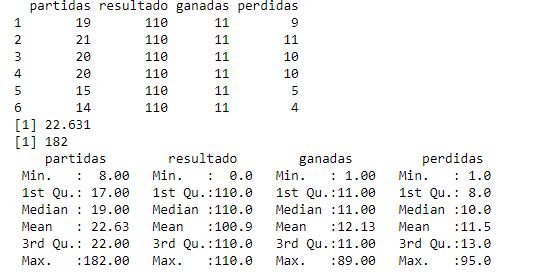
\includegraphics[scale=0.76]{i3.png}
    \caption{Tabla de valores de la muestra experimental}
    \label{fig:my_label}
\end{figure}
\begin{figure}
    \centering
    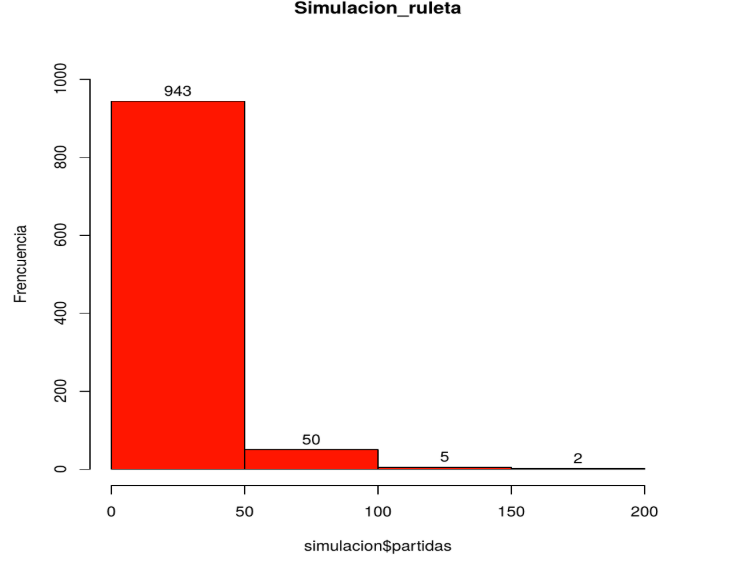
\includegraphics[scale=0.5]{i34.png}
    \caption{Histrograma que muestra la frecuencia con la cual se llega al tiempo de parada en cierta candtidad de partidas }
    \label{fig:my_label}
\end{figure}

Nuestro objetivo fijado era obtener S/. 10 partiendo de un capital inicial de S/.100 , observamos
que el promedio de partidas por cada jugada es de aproximadamente 22.631 partidas. Si miramos el histograma vemos como de las 1000 simulaciones o partidas, un 94,3\% se encuentran por
debajo de las 50 partidas.
Si calculamos el número de partidas en las que logramos el objetivo mediante las simulaciones
del método de la Martingala, obtenemos un 87.69 \% .

\newpage
Compararemos el resultado anterior con el nuestro  que en vez de apostar S/.1  se apuesta una cantidad de S/.17 .Es evidente que no lograremos
la cantidad deseada pues no llegará a 110 soles a los mas llegará a S/.134
El código R que se implementa para simular 1000 juegos en los cuales el resultado es alcanzar los 110 soles o perder hasta quedar en 0 soles es 
\newpage
\begin{minted}[breaklines, frame=single, tabsize=4, gobble=0]{R}
#R version 3.3.2 
N<-1000 #simulaciones
xt<- 110 # Dinero Objetivo
simulacion <- data.frame(partidas= integer(0), resultado= integer(0), ganadas=integer(0), perdidas=integer(0))
for (i in 1:N){
x0<-100 #dinero inicial
apu<-17 # dinero que apostamos por partida
g<-1
p<-1
j<-1
while(x0>0 & x0<xt){ # & apu<=x0
resultado<-runif(1,0,1)
if(x0<apu){apu = x0}
if(resultado>=(18/37)){
x0<-x0+apu
g<-g+1
apu <- 1
}else{
x0<-x0-apu
apu<-apu*2
p<-p+1
}
j<-j+1
}
simulacion[i,1]<-j
simulacion[i,2]<-x0
simulacion[i,3]<-g
simulacion[i,4]<-p
}
simulacion
head(simulacion)
mean(simulacion$partidas)
max(simulacion$partidas)
summary(simulacion)
hist(simulacion$partidas, labels=TRUE,ylab="Frencuencia", ylim=c(0,1050), nclass=3,col="red", main="Simulacion_ruleta")


\end{minted}
\begin{figure}
    \centering
    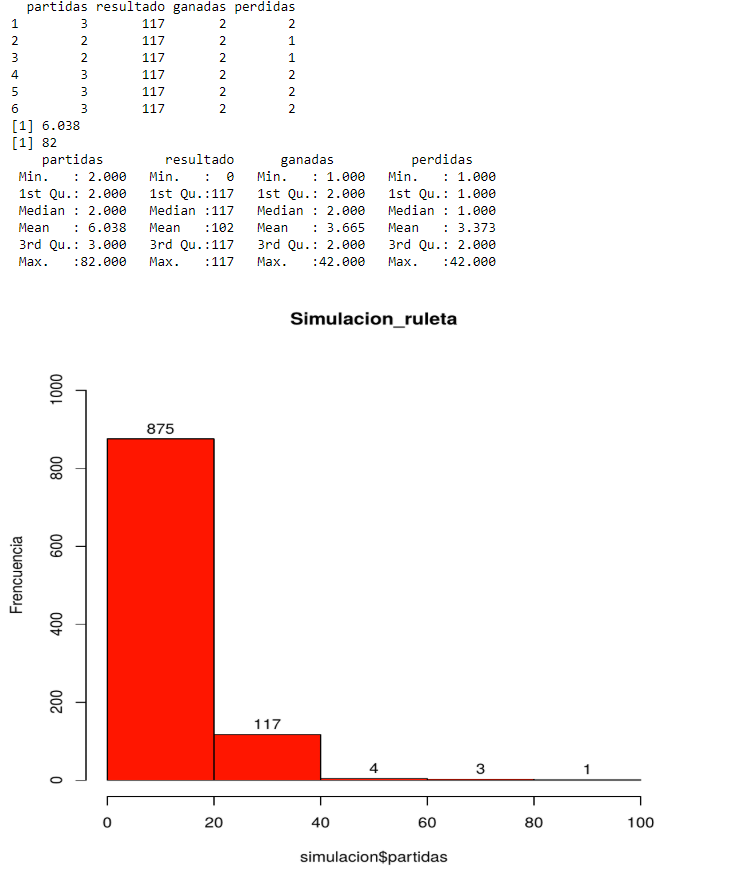
\includegraphics[scale=0.56]{312.png}
    \caption{Histograma de frecuencias cuando se comienza a apostar con S./17 siguiendo la estrategia de la martingala}
    \label{fig:my_label}
\end{figure}
En los resultados podemos ver como la probabilidad de ruina con estas condiciones es de
0,0654, inferior a la probabilidad teórica, aunque cada vez mas parecidas entre ellas.
En los juegos de azar regulados por salas de apuestas o casinos, hay circunstancias que son
totalmente ajenas al jugador, este es el caso de las probabilidades de acierto o fallo, el juego
es el que es, y estas probabilidades no varian. En cambio el jugador puede decidir aunque con
limitaciones sobre las cantidades que apuesta y tiene poder de decisión sobre el dinero que
quiere jugar en total.
\newpage

\begin{minted}[breaklines, frame=single, tabsize=4, gobble=0]{R}
ruina_jugador=function(u,N,p){
k=u;j=0; C=u
while(k>0&&k<N){
r=rbinom(1,1,p)
e=2*r-1; y=k+e; k=y; j=j+1
C=c(C,k)}
plot(0:j,C,type="o",ylim=c(0,N))
abline(h=c(0,N),v=c(0,j))
a=j/2; b=.8*N
text(a,b,labels=paste('Num. Apuestas =',j),pos=3,cex=2,col="blue")
j}
##EJEMPLO
ruina_jugador(2,100,.486)
[1] 172
\end{minted}
\begin{figure}
    \centering
    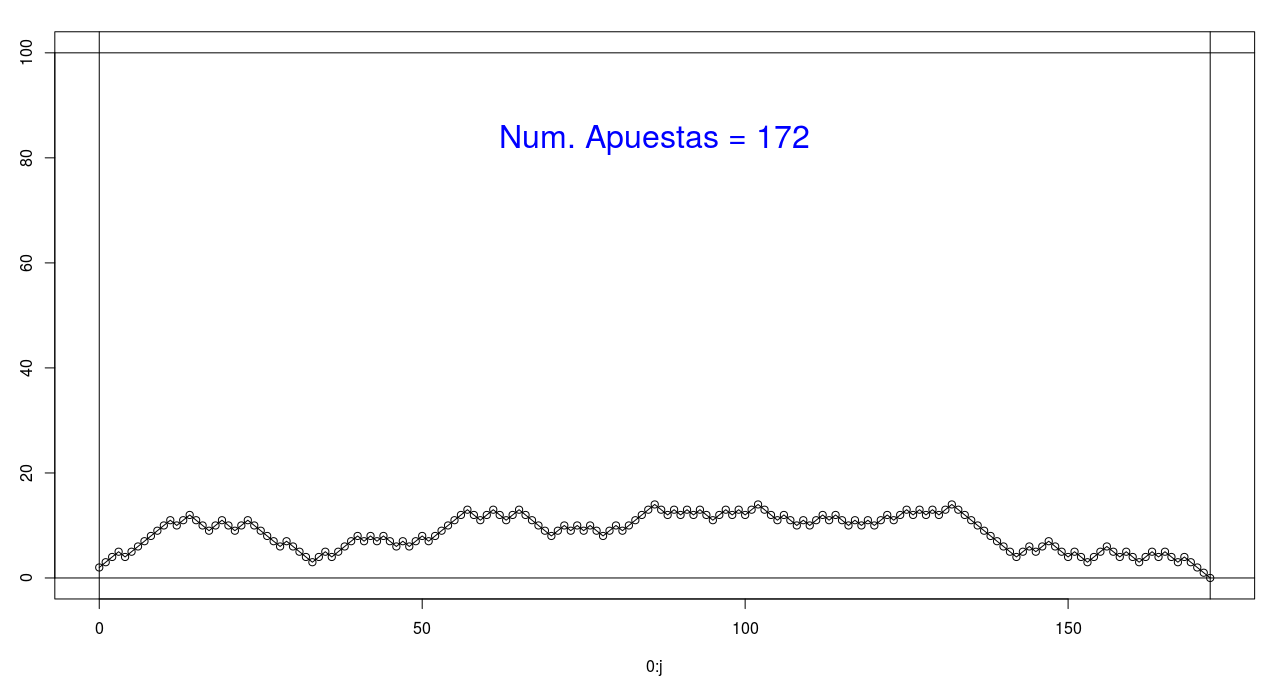
\includegraphics[scale=0.3]{172.png}
    \caption{Polígono de frecuencias para 172 apuestas}
    \label{fig:my_label}
\end{figure}








%\newpage
%LINEA BASE REPRODUCCION DE RESULTADOS, EVALUACION DEL RENDIMIENTO Y COMPARACION DE LINEA BASE Y RESULTADOS PROPIOS
%\begin{center}
%\textbf{DISCUSIÓN}  




%\end{center}
%INTERPREATCION DE LOS RESULTADOS Y COMO PODRIA MEJORAR NUESTROS RESULTADOS
%\begin{center}
%\textbf{CONCLUSIONES}  
%\end{center}
%LAS CONCLUSIONES SOBRE Y LOS TEOREMAS QUE  DEMOSTRAMOS                                                 




%\section{Diseño del experimento}\label{sec:3}



\begin{itemize}

\end{itemize}








%\begin{table}[h]
%\caption{An Example of a Table}
%\label{table_example}
%\begin{center}
%\begin{tabular}{|c||c|}
%\hline
%One & Two\\
%\hline
%Three & Four\\
%\hline
%\end{tabular}
%\end{center}
%\end{table}


  % \begin{figure}[thpb]
   %   \centering
  %    \framebox{\parbox{3in}{We suggest that you use a text box to insert a graphic (which is ideally a %300 dpi TIFF or EPS file, with all fonts embedded) because, in an document, this method is somewhat %more stable than directly inserting a picture.
%}}
 %     %\includegraphics[scale=1.0]{figurefile}
 %     \caption{Inductance of oscillation winding on amorphous
 %      magnetic core versus DC bias magnetic field}
  %    \label{figurelabel}
  % \end{figure}
   




%\addtolength{\textheight}{-12cm}   % This command serves to balance the column lengths
                                  % on the last page of the document manually. It shortens
                                  % the textheight of the last page by a suitable amount.
                                  % This command does not take effect until the next page
                                  % so it should come on the page before the last. Make
                                  % sure that you do not shorten the textheight too much.

%%%%%%%%%%%%%%%%%%%%%%%%%%%%%%%%%%%%%%%%%%%%%%%%%%%%%%%%%%%%%%%%%%%%%%%%%%%%%%%%



%%%%%%%%%%%%%%%%%%%%%%%%%%%%%%%%%%%%%%%%%%%%%%%%%%%%%%%%%%%%%%%%%%%%%%%%%%%%%%%%



%%%%%%%%%%%%%%%%%%%%%%%%%%%%%%%%%%%%%%%%%%%%%%%%%%%%%%%%%%%%%%%%%%%%%%%%%%%%%%%%

\newpage

\begin{thebibliography}{99}

\bibitem{c1} M. Loeve, Probability theory II (Book graduate texts in Mathematics), Ed.  Iberica: Springer-Verlag © 1978

\bibitem{c2}Williams, David (1991). Probability with Martingales. Cambridge University Press. ISBN 0-521-40605-6.
\bibitem{c4} H. Poor, An Introduction to Signal Detection and Estimation.   New York: Springer-Verlag, 1985, ch. 4.
 Chicago, IL.
 \bibitem{c5} Giraldo. G. Norman. Procesos Estocásticos.Universidad Nacional de Colombia. Medellín. 2006. 
\bibitem{c6} Marc Martínez, Xavier Bardina. Cadenas de Markov:
Estudio sobre el problema de la ruina del jugador. Universidad autónoma de Barcelona. España. 2017.


\end{thebibliography}




\end{document}
© 2018 GitHub, Inc.
Terms
Privacy
Security
Status
Help
Contact GitHub
Pricing
API
Training
Blog
About
